\documentclass{article}
\usepackage{tikz}
\usetikzlibrary{shapes, arrows.meta, positioning, shapes.geometric}
\usepackage{amsmath}
\usepackage{amssymb}
\tikzstyle{process} = [rectangle, 
minimum width=1.5cm, 
minimum height=0.8cm, 
text centered, 
text width=2cm, 
draw=black, 
fill=orange!30]

\tikzstyle{decision} = [diamond, 
minimum width=1.5cm, 
minimum height=0.8cm, 
text centered, 
draw=black, 
fill=green!30]
\tikzset{
    %process/.style = {rectangle, draw, text width=6em, text centered, minimum height=1.5em},
    %decision/.style = {diamond, draw, text width=5.5em, text centered, aspect=2, minimum height=1.5em},
    answer/.style = {rectangle, draw, text width=2em, text centered, minimum height=1em, fill=gray!20},
    arrow/.style = {thick, -Stealth}
}

\begin{document}
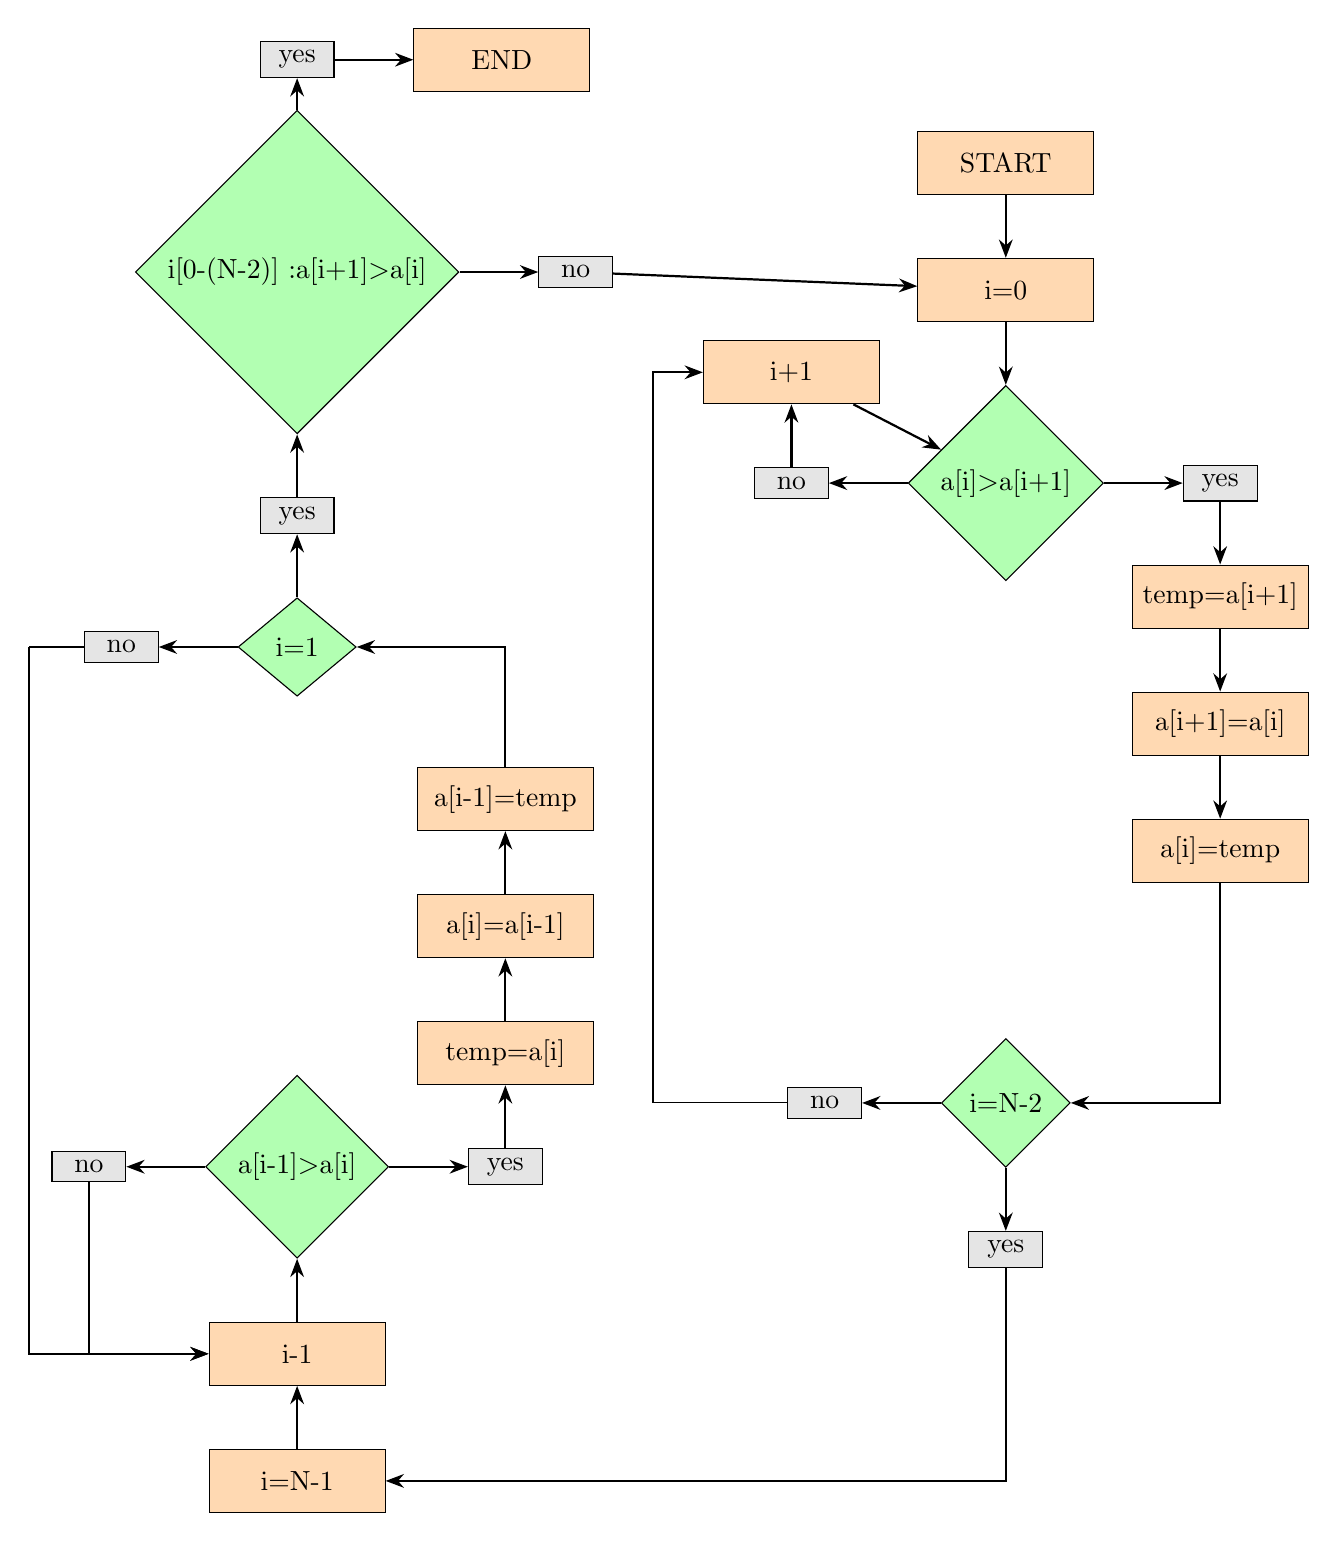
\begin{tikzpicture}[xshift={(-3cm)}, node distance=0.8cm and 1cm]
%Nodes 
\node (process) [process] {START};
\node (process1) [process, below=of process] {i=0};
\node (decision) [decision, below=of process1] {a[i]\textgreater a[i+1]};
\node (no) [answer, left=of decision] {no};
\node (process2) [process, above=of no] {i+1};
\node (yes) [answer, right=of decision] {yes};
\node (process3) [process, below=of yes] {temp=a[i+1]};
\node (process4) [process, below=of process3] {a[i+1]=a[i]};
\node (process5) [process, below=of process4] {a[i]=temp};
\node (decision2) [decision, below=of decision, yshift=-5cm] {i=N-2};
\node (no2) [answer, left=of decision2] {no};
\node (yes2) [answer, below=of decision2] {yes};
\node (process6) [process, below=of yes2, xshift=-9cm, yshift=-1.5cm ] {i=N-1};
\node (process7) [process, above=of process6] {i-1};
\node (decision3) [decision, above=of process7] {a[i-1]\textgreater a[i]};
\node (yes3) [answer, right=of decision3] {yes};
\node (no3) [answer, left=of decision3] {no};
\node (process8) [process, above=of yes3] {temp=a[i]};
\node (process9) [process, above=of process8] {a[i]=a[i-1]};
\node (process10) [process, above=of process9] {a[i-1]=temp};
\node (decision4) [decision, above=of decision3, yshift=4cm] {i=1};
\node (no4) [answer, left=of decision4] {no};
\node (yes4) [answer, above=of decision4] {yes};
\node (decision5) [decision, above=of yes4] {i[0-(N-2)] :a[i+1]\textgreater a[i]};
\node (yes5) [answer, above=of decision5, yshift=-0.4cm] {yes};
\node (no5) [answer, right=of decision5] {no};
\node (process11) [process, right=of yes5] {END};





%ARrrows
\draw [arrow] (process) -- (process1);
\draw [arrow] (process1) -- (decision);
\draw [arrow] (decision) -- (no);
\draw [arrow] (no) -- (process2);
\draw [arrow] (process2) -- (decision);
\draw [arrow] (yes) -- (process3);
\draw [arrow] (process3) -- (process4);
\draw [arrow] (process4) -- (process5);
\draw [arrow] (decision) -- (yes);
\draw [arrow] (process5) |- (decision2);
\draw [arrow] (decision2) -- (no2);
\draw [arrow] (decision2) -- (yes2);
\draw [] (no2) -- ([xshift=-1.7cm]no2.west);
\draw [arrow] ([xshift=-1.7cm]no2.west) |- (process2);
\draw [arrow] (yes2.south) |- (process6.east);
\draw [arrow] (process6) -- (process7);
\draw [arrow] (process7) -- (decision3);
\draw [arrow] (decision3) -- (no3);
\draw [arrow] (decision3) -- (yes3);
\draw [arrow] (no3) |- (process7);
\draw [arrow] (yes3) -- (process8);
\draw [arrow] (process8) -- (process9);
\draw [arrow] (process9) -- (process10);
\draw [arrow] (process10) |- (decision4);
\draw [arrow] (decision4) -- (yes4);
\draw [arrow] (decision4) -- (no4);
\draw [arrow] ([xshift=-0.7cm]no4.west) |- (process7);
\draw [] (no4.west) -- ([xshift=-0.7cm]no4.west);
\draw [arrow] (yes4) -- (decision5);
\draw [arrow] (decision5) -- (yes5);
\draw [arrow] (decision5) -- (no5);
\draw [arrow] (no5) -- (process1);
\draw [arrow] (yes5) -- (process11);



\end{tikzpicture}
\end{document}